\documentclass{article}
\usepackage[utf8]{inputenc}
\usepackage{amsfonts}
\usepackage{amsmath}
\usepackage{hyperref}
\usepackage{graphicx}
\usepackage[export]{adjustbox}
\usepackage{xcolor}
\usepackage{caption}
\usepackage[section]{placeins}
\captionsetup[figure]{name=Slika}
\renewcommand\refname{Viri in literatura}

\title{Končno poročilo projekta: Igra 2048}
\author{Maj Gaberšček}
\date{Ljubljana, april 2022}

\begin{document}

\maketitle

\section{Uvod}
Pri predmetu Matematika z računalnikom si je vsak študent izbral svoj projekt med projekti, ki so vključevali projekte raznih industrijskih panog, projekte iz optimizacije, teorije iger,... Sam sem si izbral projekt z naslovom \emph{Games 3: 2048}. V sklopu projekta sem si zastavil nalogo, da uspešno zasnujem uporabniški vmesnik za igranje igre 2048. Ta bo uporabniku omogočal, da sam odigra igro, ali pa izbere računalniški algoritem, ki nato odigra igro in jo skuša premagati. Mogoča je tudi kombinacija: igralec odigra igro do neke poteze, potem pa jo naprej skuša rešiti računalnik, ali obratno. Za implementacijo sem si izbral programski jezik \texttt{Java}, ki s knjižnico \texttt{Swing} omogoča relativno preprosto implementacijo uporabniškega vmesnika. Projekt sem sproti objavljal tudi na repozitorij na \texttt{Githubu}.

\section{Predstavitev igre 2048}

\subsection{Predstavitev}

2048 je enoigralska video igra, ki jo je izumil italijanski razvijalec Gabriele Cirulli leta 2014 in jo objavil na \texttt{Github}. Cilj igre je skupaj sestavljati različne številke na mreži in doseči število 2048. Mreža je praviloma velikosti 4x4, čeprav se v različnih variantah igre pojavlja tudi v drugih velikostih (na primer 3x3 ali 5x5) \cite{wiki:2048_(video_game)}. V teoriji iger je sicer dokazano, da je problem igre 2048 NP-poln.\cite{DBLP:journals/corr/AbdelkaderAD15}

\subsection{Pravila}

Uporabnik lahko, ko je na vrsti, naredi potezo, pri čemer ima ponavadi na voljo 4 različne: premik gor, premik dol, premik levo in premik desno. Ob premiku v želeno smer se vsako število premakne najdlje možno v tisto smer, dokler ni zaustavljeno ali s koncem mreže, ali z drugo številko. Pri tem se, če se zaletita dve enaki števili, združita v novo število, ki je vsota obeh (dvakratnik). Upoštevati moramo, da se, v kolikor se zaletijo tri enaka števila, v dvakratnih združita samo tisti dve, ki sta najdlje v smeri premika. Poteze, ki mreže ne spremeni (torej ostane enaka kot pred premikom), ne smemo odigrati.

Po vsakem premiku se na naključno prazno mesto na mreži pojavi novo število, ki je 2 z verjetnostjo 90\% in 4 z verjetnostjo 10\%.

Igra je izgubljena, ko uporabnik nima več možnih potez, torej nobena poteza ne spremeni mreže. Če uporabnik doseže število 2048, je igro premagal. Večina aplikacij sicer uporabniku omogoča tudi igranje naprej po zmagi. Z ustrezno strategijo je namreč igro precej preprosto premagati.

\subsection{Točkovanje}

Igra ponuja tudi točkovanje. Po zmagi je namreč cilj uporabnikov to, da dosežejo čim več točk.

Točke se zbirajo tako, da se vsakič, ko se dve števili združita v njuno vsoto, le-ta prišteje točkam.

\subsection{Strategija človeka}

Ljudje, ki igro igrajo, ponavadi uporabijo strategijo, da največje število na mreži hranijo v določenem kotu, zraven nje pa ostala velika števila, pri čemer je cilj predvsem v tem, da največje število ne skoči iz kota.

Potrebno je tudi poudariti, da igre seveda ni mogoče igrati v nedogled. Največje število, ki ga lahko z idealno igro in precej sreče (samo teoretično) dosežemo, je 131072.

\section{Načrt dela}

Najprej sem v programskem jeziku \texttt{Java} ustvaril razred \texttt{Game.java}, ki predstavlja igro. Na razredu sem implementiral metode, ki služijo premikom, pojavitvam novih števil,...

Nato sem s pomočjo knjižnice \texttt{Swing} definiral dva nova razreda. Razred \texttt{Panel.java} je nekakšno platno, ki služi za risanje igre in podpira interakcijo uporabnika s tipkami (premiki na igri) Razred \texttt{Frame.java} je okno, ki vsebuje platno. Okno vsebuje tudi menijsko vrstico, s pomočjo katere izbiramo med nastavitvami igre in igralci.

Zadnji korak je vključeval zasnovo algoritmov, ki (uspešno) rešujejo igro in nato implementacija delovanja teh algoritmov na igri. Algoritmi so predstavljeni kot metode na razredu \texttt{Game.java}, pri čemer klic metode odigra potezo, ki jo posamezen algoritem izbere. Algoritmi so različno uspešni, predvsem pa velja pravilo, da je uspešnost algoritmov ponavadi obratno sorazmerna s časom na potezo. 

\section{Uporabniški vmesnik}

\begin{figure}[ht!]
\centering
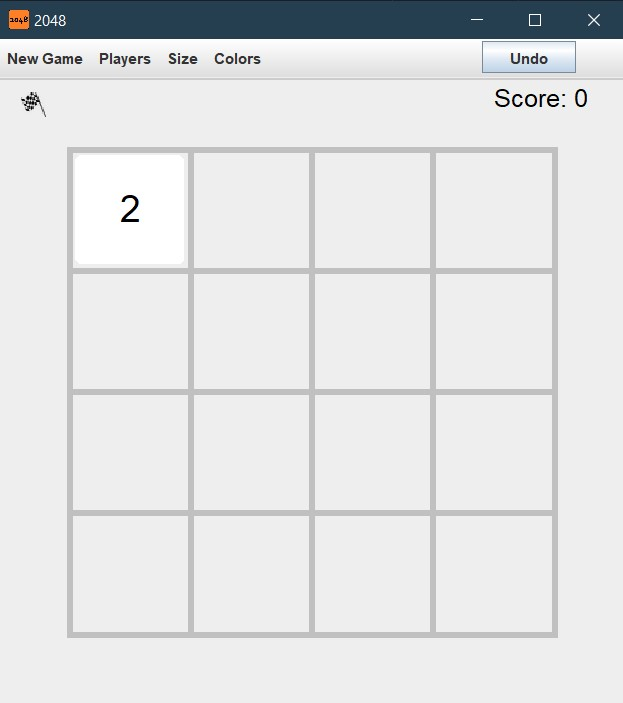
\includegraphics[width=8cm]{ui.jpg}
\caption{Posnetek zaslona uporabniškega vmesnika, ko aplikacijo zaženemo}
\label{ui}
\end{figure}

Na Sliki \ref{ui} je posnetek zaslona uporabniškega vmesnika aplikacije. Kot lahko vidimo, se čez večino okna nariše mreža (v primeru klasične igre je velikosti 4x4). Vsakič, ko aplikacijo zaženemo, se privzeto pojavi nova igra velikosti 4x4, ki jo lahko igramo. 

Zgoraj desno imamo napis \emph{Score}, ki nam sporoča trenutno število točk, ki smo jih dosegli. Zgoraj levo je ikonica, ki nam sporoča, kateri način igre trenutno igramo. V aplikacijo sem sprogramiral dva načina igranja: način \emph{Classic}, ki pomeni, da se igra konča, ko dosežemo število 2048, ter način \emph{Endless}, ki omogoča igranje, dokler ne izgubimo. Način igranja izberemo v menijski vrstici, pod zavihkom \emph{New Game}.

V menijski vrstici lahko pod zavihkom \emph{Players} izbiramo igralca. Izberemo lahko igralca \emph{Player} in potem igro igramo sami, ali pa izberemo igralca \emph{Computer}. V slednjem primeru bo izbrani računalniški algoritem (ki ga izberemo pod zavihkom \emph{Computer Algorithm}) poskušal odigrati igro. Če želimo med igro spremeniti igralca, samo izberemo drugega igralca v tem podmeniju. Na primer, aplikacija omogoča, da računalnik odigra do neke poteze in potem naprej odigramo mi ali obratno.

V zavihku \emph{Size} v menijski vrstici izbiramo velikost mreže igre. Pri tem je potrebno paziti, saj se vsaka sprememba odraža v novi igri (staro igro izgubimo). Implemenirane so velikosti igre 3x3, 4x4, 5x5, 6x6 in 8x8.

Zavihek \emph{Colors} nam omogoča, da si izberemo barvno shemo, ki spremeni barve. Barvne sheme lahko menjamo med igranjem, brez da to vpliva na igro.

Desno od menijske vrstice je še gumb z napisom \emph{Undo}, ki služi razveljavitvi poteze. Medtem, ko igra računalnik, gumb ne deluje. Prav tako med igranjem računalnika tudi ne delujejo tipke, ki odigravajo človekove poteze (w, a, s in d). Zavedam se, da gumb \emph{Undo} lahko uporabljamo za goljufanje igre (manipuliramo kje na mreži se bo pojavila nova številka). Vseeno je tak gumb koristen, če na primer po pomoti odigramo potezo, ki je nismo želeli odigrati.

Okno z igro je spremenjive velikosti, vendar igra 4x4 najlepše izgleda v privzeti velikosti. Če okno preveč pomanjšamo, bodo številke postale prevelike za prikaz na mreži in se jih ne bo videlo.

\section{Računalnikovi algoritmi}

Implementiral sem štiri različne računalnikove algoritme za reševanje igre, ki so med seboj različno uspešni.

\subsection{Algoritem \texttt{Random moves}}

Kot nam že ime samo po sebi pove, ta algoritem uporablja naključne poteze za reševanje igre. Algoritem sicer ni pretirano uspešen, je pa podlaga za bolj uspešna in kompleksna algoritma, opisana v naslednjih dveh podpoglavjih.

\subsection{Algoritem \texttt{Simulator(k)}}

Ta algoritem je v teoriji iger znan kot \textbf{Pure Monte Carlo game search}. Algoritem sprejme naravno število $k$. Nato določi vse možne poteze, ki jih v dani poziciji na mreži lahko odigra. Za vsako izmed teh nato v ozadju odigra $k$ naključnih iger, kjer najprej odigra izbrano potezo, nato pa dokonča igro z algoritmom \texttt{Random moves}, ki je opisan v prejšnjem podpoglavju, dokler ne izgubi. Nato primerja igre različnih potez in izbere tisto potezo, katere igre (simulacije) so v povprečju dosegle največje število točk, preden so izgubile.

Na primer, v dani poziciji sta možni potezi \emph{Premik gor} in \emph{Premik desno}. Recimo, da uporabimo število $k=10$. Algoritem v ozadju ustvari 10 kopij igre in na vsaki od njih najprej odigra potezo \emph{Premik gor}. Nato vse igre dokonča z algoritmom \emph{Random moves}. Algoritem v neko spremenjivko shrani povprečno število točk, ki jih je dosegel pri teh 10 igrah. Nato postopek ponovi za potezo \emph{Premik desno}. Ustvari 10 kopij originalne igre in na njih odigra \emph{Premik desno}, ter igre dokonča z naključnimi potezami, dokler ne izgubi vsake. Spet si v drugo spremenljivko shrani povprečno število točk na teh 10 igrah. Nato primerja povprečno število točk za potezo \emph{Premik gor} in \emph{Premik desno}. Odigra tisto, ki je v povprečju dosegla več točk.

\subsection{Algoritem \texttt{Dynamic simulator}}

\texttt{Dynamic simulator} je algoritem, ki je izboljšava algoritma \texttt{Simulator}. Ta ima namreč problem, da za nezahtevne pozicije porabi preveč časa, da izračuna potezo. Največ težav imajo vsi algoritmi tik pred tem, da izgradijo novo največjo številko, saj je takrat na mreži največ zasedenih polj. Na primer, preden algoritem zgradi število 2048, mora imeti na mreži že števila 1024, 512, 256, 128, 64. Takoj po tem ko število 2048 zgradi, ima vsa polja na mreži prosta, razen tistega z 2048. Torej bo precej večja verjetnost, da izgubimo tik pred izgradnjo novega najvišjega števila, kot takoj po tem. 

Zato je \texttt{Dynamic simulator} sestavljen tako, da glede na stanje na mreži ustrezno prilagaja število $k$ algoritma \texttt{Simulator(k)}. Če je pozicija bolj zahtevna, uporabimo večji $k$ (in je poteza bolj časovno zahtevna). Če pa je pozicija lažja, lahko uporabimo manjši $k$. Algoritem je tako časovno manj zahteven od navadnega \texttt{Simulatorja}. Prikaz odvisnosti $k$-ja od števila točk, doseženega na igri je prikazana na grafu na Sliki \ref{dynsim}. Uspešnost tega algorima sem analiziral v poglavju \textit{6. Analiza uspešnosti}.

\begin{figure}[ht!]
\centering
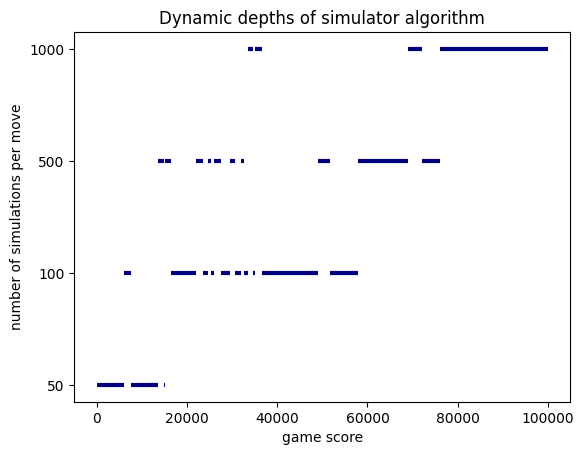
\includegraphics[width=12cm]{dynamic_sim.png}
\caption{Število simulacij na potezo v odvisnosti od točk za \texttt{Dynamic simulator}}
\label{dynsim}
\end{figure}

\subsection{Algoritem \texttt{Empty spaces}}

Ta algoritem za vsako potezo pogleda število praznih mest na mreži po njej. Izbere potezo, ki ima najmanjše število praznih polj. Če ima več potez enako število praznih mest, izbere po preferenčnem seznamu: \textit{Premik gor, Premik desno, Premik levo, Premik dol}. Algoritem sicer dobro posnema človekovo strategijo, vendar ni pretirano uspešen pri igranju. Odpove namreč v situacijah, ko je treba predvideti več kot eno potezo v naprej.

\section{Analiza uspešnosti}

Algoritmi so različno uspešni v reševanju igre in različno hitri. Za vsak algoritem in za $k \in \{1,2,5,10,15,20,50,100,500\}$ za algoritem \texttt{Simulator(k)} sem igro pognal 100-krat in analiziral uspešnost posamezega algoritma. Najprej je treba poudariti, da je hitrost \texttt{Simulatorja} linearno odvisna od števila simuliranih iger $k$. Zato hitrosti ne bom primerjal med njimi. 

Najhitrejši je algoritem naključnih potez, \texttt{Random moves}, sledi pa mu \texttt{Empty spaces}. \texttt{Simulator} je hitrejši od \texttt{Dynamic simulatorja} za manjše $k$-je, za večje pa je kar precej počasnejši.

Uspešnost algoritmov glede na povprečno največje dosežene točke, je prikazan na Sliki \ref{score}. Čeprav je \texttt{Dynamic simulator} malce slabši od \texttt{Simulatorja(500)}, pa je več kot štirikrat hitrejši. V povprečju \texttt{Simulator(500)} rabi za dosego števila 2048 približno 210 sekund, pri čemer \texttt{Dynamic simulator} igro v povprečju premaga v manj kot 40 sekund.

\begin{figure}[ht!]
\centering
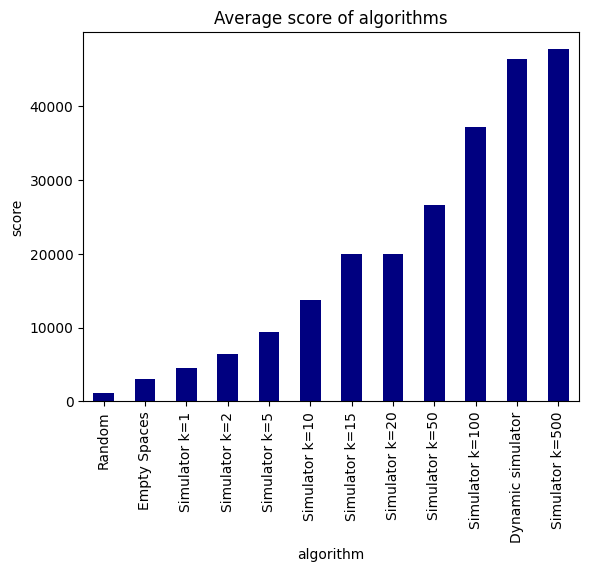
\includegraphics[width=12cm]{score.png}
\caption{Povprečno število točk, glede na posamezen algoritem}
\label{score}
\end{figure}

Najpomembnejši kazalec uspešnosti algoritmov je, glede na naravo naloge, uspešnost pri premagovanju igre. Uspešnost \texttt{Simulatorja} prikazuje graf \ref{performance}. Algoritma \texttt{Random moves} in \texttt{Empty Spaces} v 100 poskusih igre nista uspela premagati. Algoritem \texttt{Dynamic Simulator} je igro premagal 92-krat od 100 poskusov.

\begin{figure}[ht!]
\centering
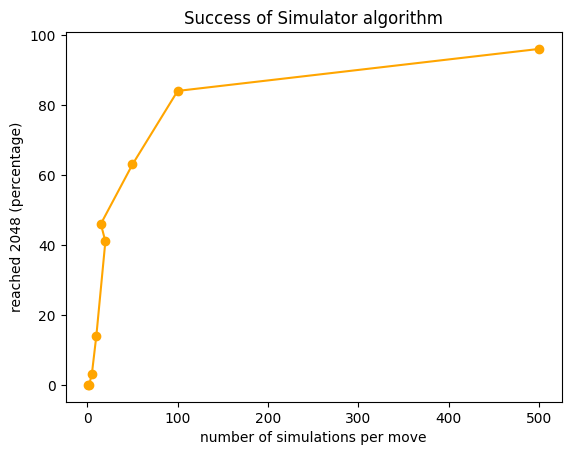
\includegraphics[width=12cm]{simulator.png}
\caption{Odvisnost števila simulacij od uspešnosti za \texttt{Simulator}}
\label{performance}
\end{figure}

Nekako se zdi, da uspešnost logaritemsko narašča s številom simulacij. Za boljši pregled odvisnosti bi bilo potrebno testirati tudi vrednosti med $k=100$ in $k=500$, ter povečati število simulacij. Tega nisem storil, saj je moj računalnik že tako ogromno časa porabil za reševanje 100 iger \texttt{Simulatorja(500)}.

Kot sem že prej poudaril, je po uspešnosti \texttt{Dynamic simulator} najbližje \texttt{Simulatorju(500)}, a je precej hitrejši. \texttt{Dynamic simulator} bi lahko bil prilagojen tako, da bi igro reševal bolje, vendar sem se zadovoljil z 92\% uspešnostjo in zelo hitrim reševanjem.

\pagebreak
\section{Posnetki zaslona}

\begin{figure}[ht!]
\centering
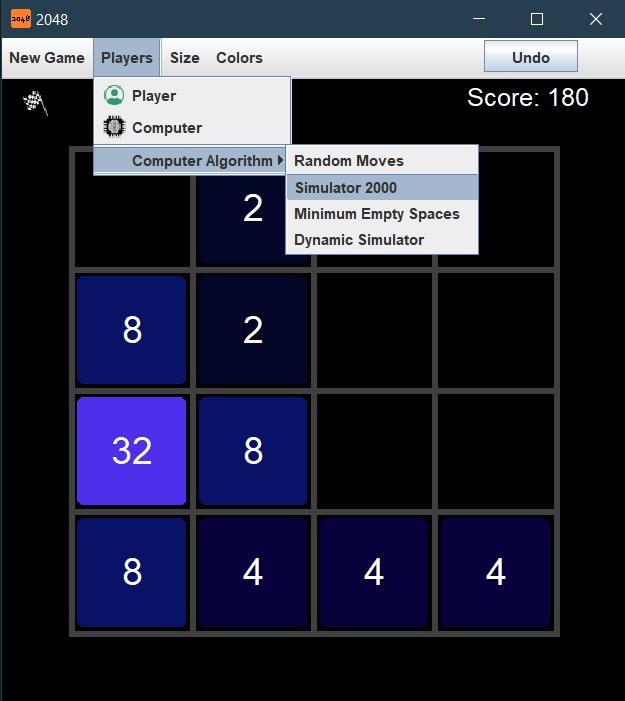
\includegraphics[width=6.5cm]{scr1.jpg}
\caption{Temna tema in izbiranje računalnikovega algoritma}
\label{scr1}
\end{figure}

\begin{figure}[ht!]
\centering
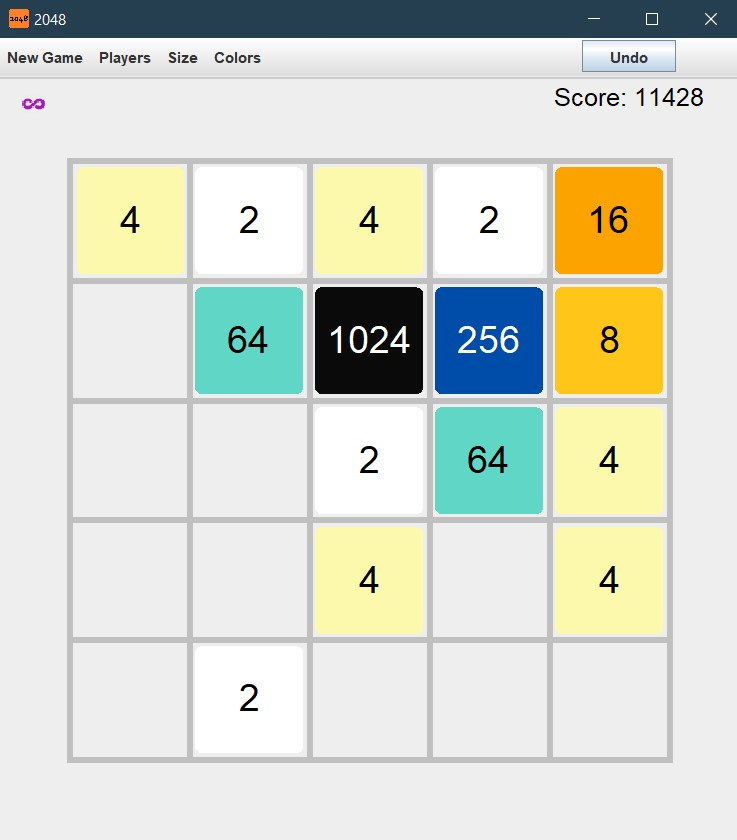
\includegraphics[width=6.5cm]{scr2.jpg}
\caption{Igra velikosti 5x5 v \emph{Endless} načinu (ikona zgoraj levo)}
\label{scr2}
\end{figure}

\begin{figure}[ht!]
\centering
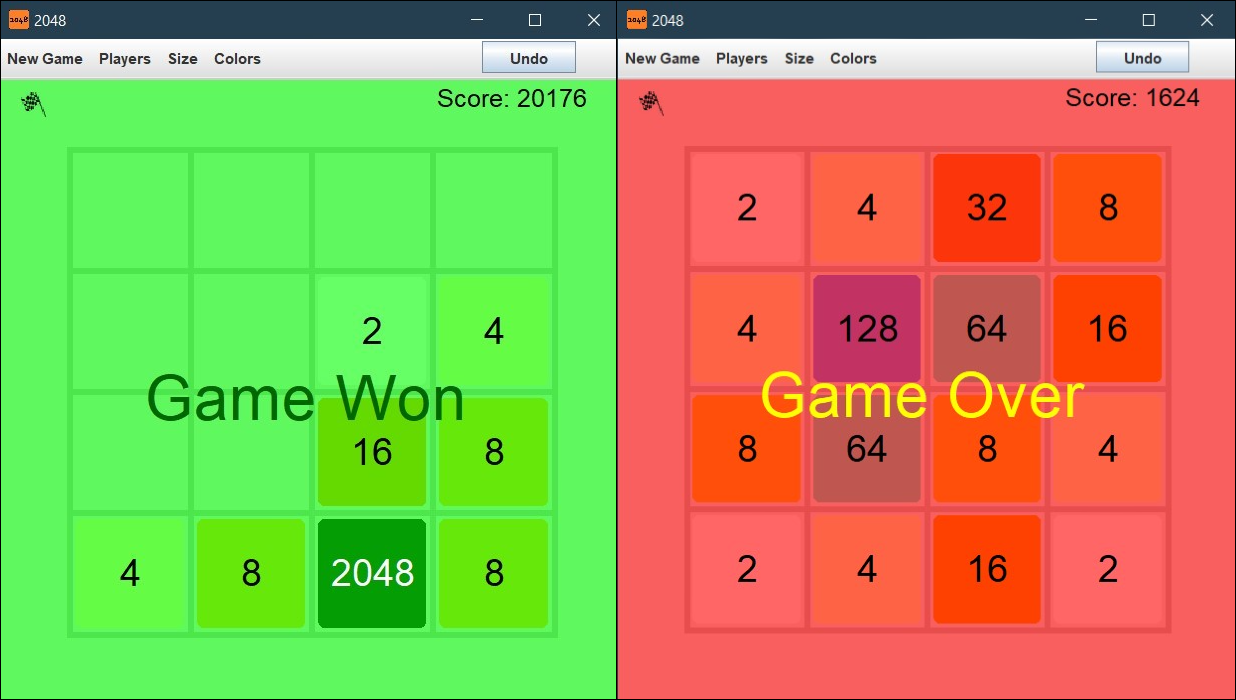
\includegraphics[width=11cm]{scr3.png}
\caption{Posnetek okna v primeru zmage (levo) in v primeru poraza (desno)}
\label{scr3}
\end{figure}

\begin{figure}[ht!]
\centering
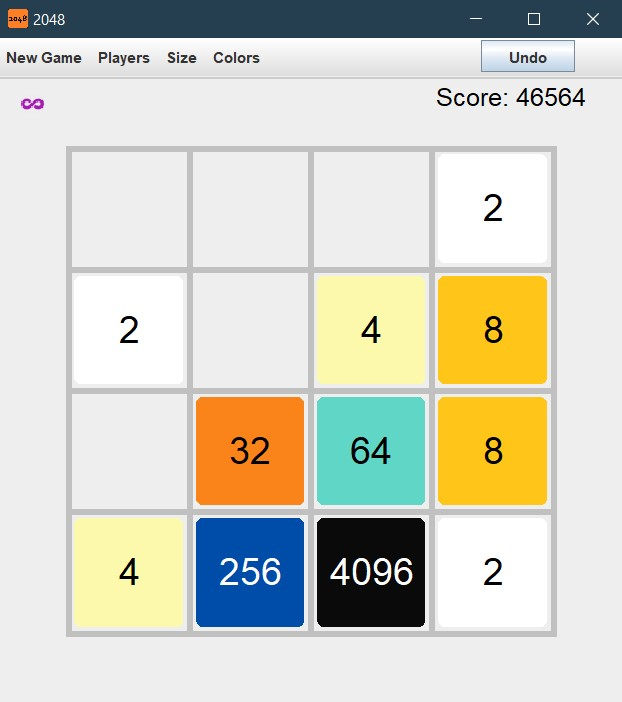
\includegraphics[width=6.5cm]{scr4.jpg}
\caption{V \emph{Endless} načinu lahko dosežemo tudi večja števila kot 2048}
\label{scr4}
\end{figure}


\section{Zaključek}

Cilj te naloge je bilo ustvariti delujočo aplikacijo, ki ponuja uporabniško izkušnjo, ter nekaj različno dobrih in hitrih računalniških algoritmov. Mislim, da mi je to do neke mere uspelo, algoritem \texttt{Dynamic simulator} je dokaj hiter in dokaj uspešen. Če bi želeli še izboljšati uspešnost, bi lahko povečali $k$ v algoritmu \texttt{Simulator(k)}. Na primer, vemo, da algoritem vedno premaga igro za $k=10000$ \cite{stackoverflow}, vendar nihče noče čakati več sekund za posamezno potezo, saj je to zelo dolgočasno. Igra potem traja več kot pol ure. Zato sem se zadovoljil z zelo verjetno zmago in raje hitrejšim časom. Glede izboljšav aplikacije sem lahko najbolj kritičen glede uporabniške izkušnje. Igra bi precej bolje izgledala, če bi vsaka poteza imela animacijo, kot na primer originalna igra Gabrieleja Cirullija, kjer se številke premaknejo iz začetnega mesta pred potezo na končno mesto po potezi. Vseeno sem ocenil, da bi kaj takšnega vzelo preveč časa in sem se zato raje osredotočil na algoritme, analizo in korektno delovanje aplikacije.

\addcontentsline{toc}{chapter}{Viri in literatura}
\bibliographystyle{unsrt}
\bibliography{literature}

\end{document}
